\section{Secret Key Cryptography}


\subsubsection{Perfect Secrecy}

\begin{theorem}{Perfect Secrecy}
    Ein Verschlüsselungsalgorithmus hat perfect secrecy, wenn für alle möglichen Plaintexte $p$ und Ciphertexte $c$ und für alle Schlüssel $k$ gilt:
    \begin{equation}
        P[p|c] = P[p]
    \end{equation}
    Das heisst, dass die Wahrscheinlichkeit, dass ein bestimmter Plaintext $p$ verschlüsselt wurde, gleich gross ist, wie die Wahrscheinlichkeit, dass ein beliebiger Plaintext $p$ verschlüsselt wurde.
\end{theorem}

\begin{concept}{One-Time-Pad} Vernam Cipher (a.k.a. One-Time-Pad)
    \begin{itemize}
        \item \textbf{Voraussetzung:} Der Schlüssel ist komplett zufällig und genau gleich lang, wie die zu verschlüsselnde Nachricht.
        \item \textbf{Verschlüsselung:}
        Der Plaintext wird mit dem Schlüssel bitweise ver-xor-ed
        $c_j = p_j \oplus k_j \forall j \in \{1, \dots, n\}$
    \end{itemize}
    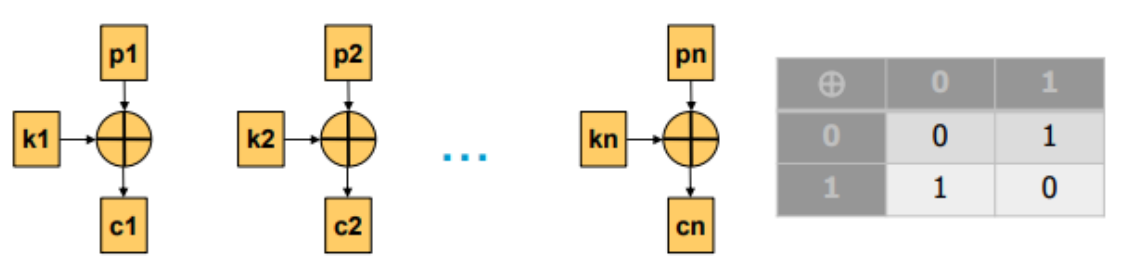
\includegraphics[width=0.7\linewidth]{vernam_cipher.png}
    \begin{itemize}
        \item Key $K$: Independent bits with equal probability
        \item $C_X = K_X \oplus P_X$
        \item Each key may be used once
        \item Same Key used multiple times: $P_1 \oplus P_2 = C_1 \oplus C_2$
    \end{itemize}
\end{concept}



\begin{corollary}{Nachteile des One-Time-Pad}
    Wenn ein Attacker jetzt alle Schlüssel ausprobieren würde, würde er neben vielen offensichtlich falschen Plaintexten auch viele plausible Plaintexte erhalten und wüsste daher nicht, welcher der plausiblen Plaintexte der korrekte ist.
    \vspace{2mm}\\
    Obwohl dies also genau das Verhalten ist, was wir möchten, kommt der One-Time-Pad nur in sehr seltenen Fällen zum Einsatz. Dies liegt daran, dass der Schlüssel
    \begin{itemize}
        \item genau gleich lang wie der zu verschlüsselnde Text sein muss
        \item komplett zufällig sein muss (vollständig zufällige Bitfolge)
        \item vorgängig geheim zwischen Sender und Empfänger ausgetauscht werden muss
        \item nur ein einziges mal verwendet werden darf (sonst ist er nicht mehr vollkommen zufällig und die ganze Sicherheit geht verloren)
    \end{itemize}
\end{corollary}

\begin{concept}{Eigenschaften sicherer kryptographischer Algorithmen}
    Da heute ausser dem One-Time-Pad kein Algorithmus bekannt ist, welcher als informationstheoretisch sicher gilt, werden folgende Eigenschaften für sichere Algorithmen definiert:
    \begin{itemize}
        \item Allgemein bekannt
        \item Keine Fehler bekannt
        \item Work Factor > $2^{128}$
    \end{itemize}
    Daraus lässt sich auch ableiten, dass wir als Noobs keine kryptographischen Algorithmen selber entwickeln/implementieren sollten. Stattdessen soll auf standardisierte Algorithmen zurückgegriffen werden. (Öffentlich verfügbare Libraries)
\end{concept}



\raggedcolumns
\columnbreak


\subsubsection{Modern Ciphers}

\begin{concept}{Random Oracle Model}
    \begin{itemize}
        \item Different inputs give random unrelated outputs
        \item If $A$ leads to $B$ then $A$ always leads to $B$
    \end{itemize}
\end{concept}


\begin{concept}{Modern Ciphers}
    \begin{itemize}
        \item Same key is used to encrypt and decrypt
        \item Wrong key gives high-entropy output: can tell when correct key used
        \item Good modern ciphers: key entropy $\approx$ work factor
        \item Cryptographic workhorse today: AES
    \end{itemize}
\end{concept}

\begin{remark} Properties of Modern Ciphers:
    \begin{itemize}
        \item Information-theoretical security is out of question
        \item Next best thing: computational security
        \item No cipher is known that can be proved to be computationally secure
        \item Cipher created $\rightarrow$ public review $\rightarrow$ gains acceptance
    \end{itemize}
\end{remark}


\begin{concept}{Secret Key Principle}
    The same key is used for encryption and decryption
\end{concept}

\subsubsection{Block Ciphers}

\mult{2}

\begin{definition}{Block Ciphers}
    The plaintext is usually not a multiple of the block size.
    \begin{itemize}
        \item Therefore a padding is needed.
        \item Use Block Cipher modes (ECB) / (CBC) for long messages
    \end{itemize}
\end{definition}


\begin{concept}{PKCS7 Padding} Block Padding\\
    Padding data is used to fill up the final block
    \begin{itemize}
        \item Removal of padding must be easy
        \item PKCS7:
        \begin{itemize}
            \item $n$ bytes must be filled, fill them with byte value $n$
            \item 0 bytes must be filled, add padding block with "10"
        \end{itemize}
    \end{itemize}
\end{concept}



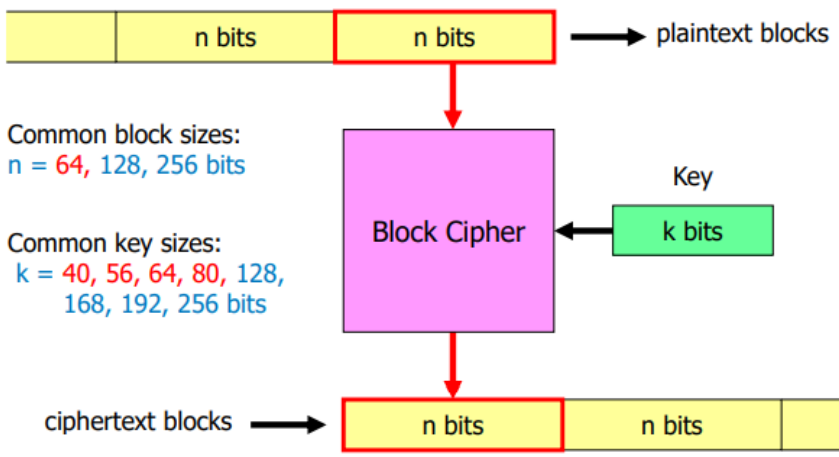
\includegraphics[width=\linewidth]{block_cipher.png}

\multend

\begin{examplecode}{PKCS7 Example}
\begin{lstlisting}[style=basesmol]
5F 6E 25 A3 36 54 90 0D D4 7F FA 05 05 05 05 05

10 10 10 10 10 10 10 10 10 10 10 10 10 10 10 10
\end{lstlisting}

0 bytes must be filled, add padding block with "10"
\end{examplecode}

\raggedcolumns
\columnbreak

\subsubsection{DES}

\mult{2}

\begin{definition}{DES (Data Encryption Standard)}
    \begin{itemize}
        \item Key size: 56 bits $\rightarrow$ totally insecure
        \item Brute force attack is still the best attack known
    \end{itemize}
\end{definition}




\begin{concept}{AES (Advanced Encryption Standard)}
    \begin{itemize}
        \item Cryptographic strength = 128 / 192 / 256
        \item Secure and modern standard
        \item Publicly defined
    \end{itemize}
\end{concept}

\begin{concept}{Triple-DES}
    \begin{itemize}
        \item Known-Plaintext Attack (MITM) $\rightarrow$ Cryptographic strength = $2^{112} + 2^{56} \approx 112$ bits
        \item Secure but relatively slow
    \end{itemize}
    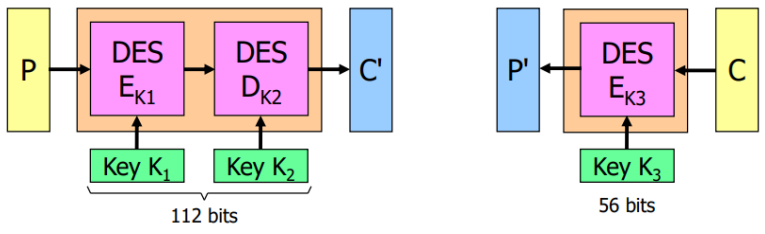
\includegraphics[width=\linewidth]{triple_DES.png}
\end{concept}

\multend

\mult{2}


\begin{definition}{ECB Mode} Electronic Code Book Mode
    \begin{itemize}
        \item Same $P$ is always same $C$
        \item Susceptible to replay attacks
        \item Patterns may remain (Pinguin)
    \end{itemize}
    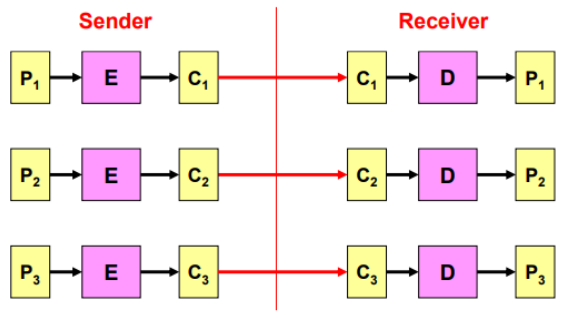
\includegraphics[width=\linewidth]{ECB.png}
\end{definition}


\begin{concept}{CBC Mode} Cipher Block Chaining Mode
    \begin{itemize}
        \item IV transmitted openly
        \item IV may only be used once
        \item Does not ensure the integrity
    \end{itemize}
    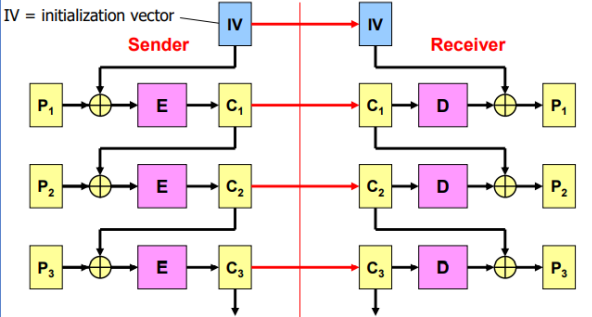
\includegraphics[width=\linewidth]{CBC.png}
\end{concept}

\multend

\mult{2}


\begin{definition}{Stream Ciphers}
    \begin{itemize}
        \item No need to wait for full block
        \item Faster than block ciphers
        \item Most stream ciphers are broken
        \item Can be implemented with block ciphers (OFB, CTR)
        \item Decryption works by reapplying the keystream: $C = P \oplus K \rightarrow P = C \oplus K$
    \end{itemize}
    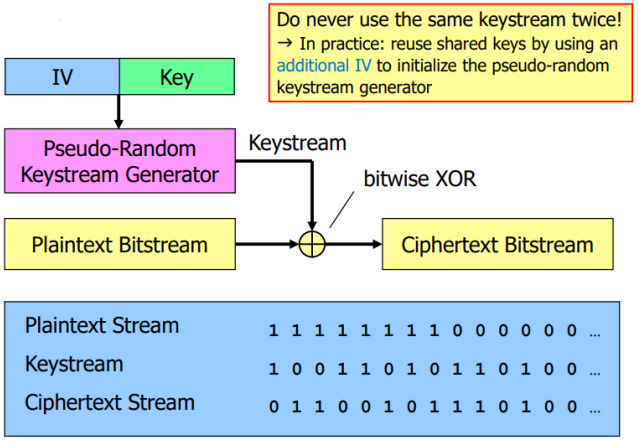
\includegraphics[width=\linewidth]{stream_ciphers.png}
\end{definition}

\begin{remark} Security of Stream ciphers
    \begin{itemize}
        \item RC4, GSM A5/1 and A5/2: Considered broken
        \item ChaCha20: Considered secure (Supported by TLS) $\rightarrow$ Today's standard
    \end{itemize}
\end{remark}


\begin{concept}{OFB Mode} Output Feedback Mode\\
    Stream cipher with block cipher\\
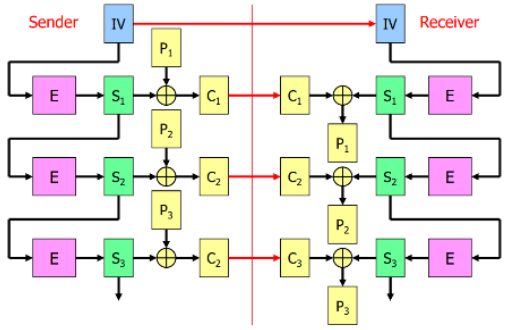
\includegraphics[width=\linewidth]{OFB.png}
\end{concept}



\begin{concept}{CTR Mode} Counter Mode
    \begin{itemize}
        \item Stream cipher with block cipher
        \item Allows for parallel encryption/decryption
    \end{itemize}
    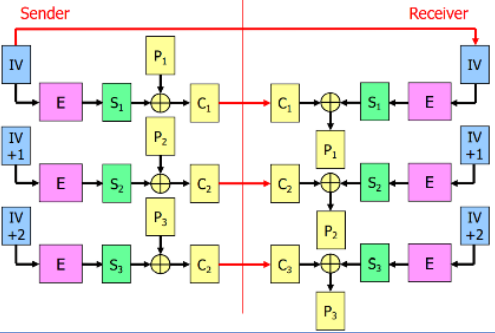
\includegraphics[width=\linewidth]{CTR.png}
\end{concept}



\multend



\raggedcolumns
\columnbreak



\section{Public Key Cryptography}

\subsection{Secure key distribution problem}

\begin{concept}{Key Distribution Problem}
    \begin{itemize}
        \item Secret key cryptography only works if the keys are exchange securely
        \item How can we obtain the key from someone unknown?
        \item How do we manage keys for large number of participants?
    \end{itemize}
    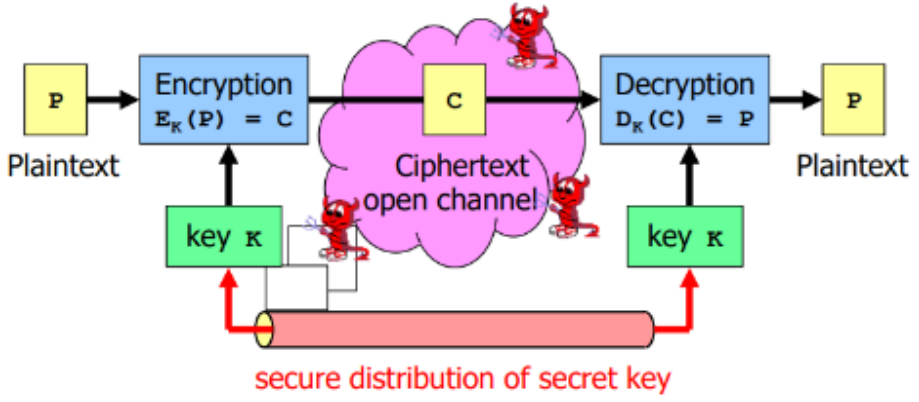
\includegraphics[width=0.5\linewidth]{key_distribution.png}
\end{concept}

\subsection{Principle of public key cryptography}

\begin{definition}{Public Key Cryptography}
    \begin{itemize}
        \item \textbf{Public Key} Known to anyone $\rightarrow$ Encryption
        \item \textbf{Private Key} Known to owner $\rightarrow$ Decryption
    \end{itemize}
\end{definition}

\begin{concept}{Properties}
    \begin{itemize}
        \item Public and Private key fit together: $D(E(M)) = M$
        \item Private key can't be computed easily from public key
    \end{itemize}
\end{concept}

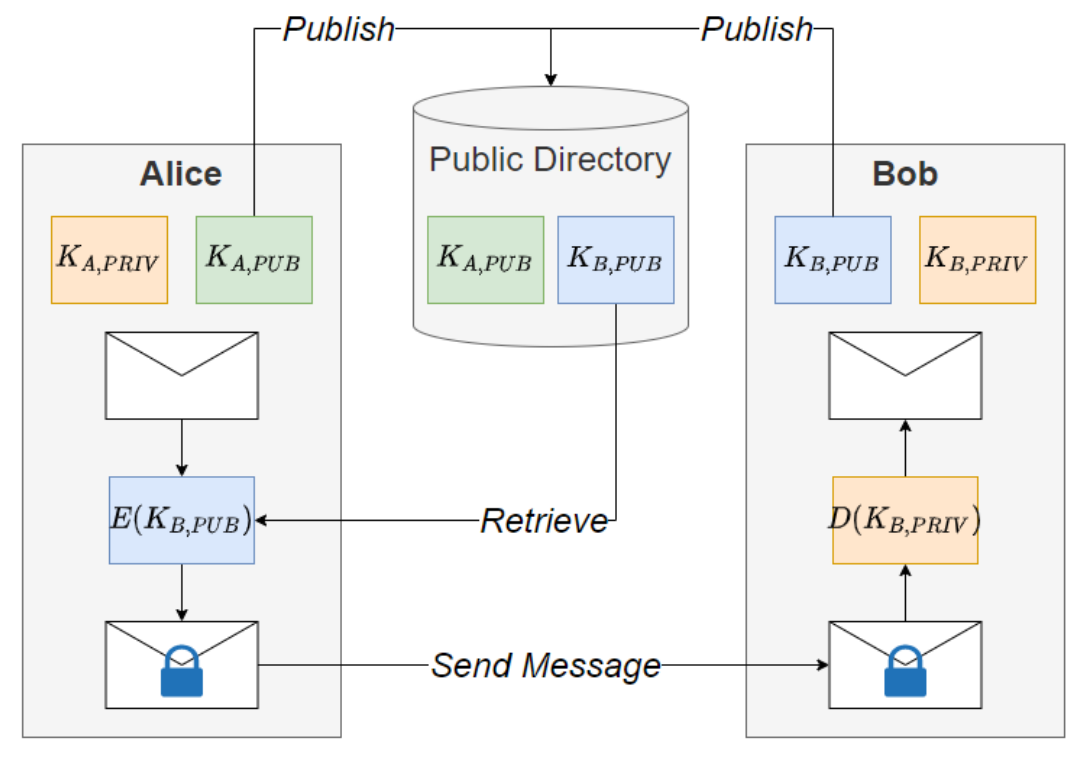
\includegraphics[width=\linewidth]{public_key.png}

\subsection{RSA (Rivest-Shamir-Adleman)}

\begin{definition}{RSA Algorithm}
    Let $(n, e)$ be RSA public key and $(n, d)$ the corresponding private key. Let $m$ be an integer with $0 \leq m < n$. Then $(m^e \bmod n)^d \bmod n = m$.
    \begin{itemize}
        \item Public Key $(n, e)$
        \item Private Key $(n, d)$
        \item $0 \leq m < n$
        \item $\varphi(n) = (q - 1) \cdot (p - 1)$
    \end{itemize}
\end{definition}

\begin{KR}{RSA Key-Pair Creation}
    \paragraph{Step 1: Choose Primes}
    Choose large primes $p, q \rightarrow pq = n$
    
    \paragraph{Step 2: Choose e}
    Choose $e$ so that $\gcd(e,\varphi(n)) = 1$
    
    \paragraph{Step 3: Compute d}
    Compute $d$ so that $ed \bmod \varphi(n) = 1$
\end{KR}

\begin{formula}{RSA Encrypt/Decrypt}
    \begin{itemize}
        \item Encrypt: $c = E(m) = m^e \bmod n$
        \item Decrypt: $m = D(c) = c^d \bmod n$
    \end{itemize}
\end{formula}

\subsection{RSA - Attacks}

\begin{definition}{RSA Attack Types}\\
    \textbf{Short message attack (Plain-Text-Attack)}
    \begin{itemize}
        \item Message $m$ is short $\rightarrow$ Ciphertext $c$ easy to decrypt
        \item Prevent by using padding for encryption
    \end{itemize}
    
    \textbf{Low public exponent attack $e$}
    \begin{itemize}
        \item $e$ is "low" and the same message $m$ is sent $e$ times
        \item Prevent by using higher values for value for $e$
    \end{itemize}
    
    \textbf{Common factor attack}
    \begin{itemize}
        \item gcd of two moduli not sharing a common prime factor = 1
        \item gcd of two moduli sharing a common prime factor $\rightarrow$ product of all
        \item If gcd = 1 $\rightarrow$ no common primes, else $p = gcd$
        \item If $p$ has been found: $n/p = q$
    \end{itemize}
\end{definition}

\subsection{Groups}

\begin{definition}{Mathematical Groups}\\
    A group $(G, \circ)$ has the following properties:
    \begin{itemize}
        \item $\circ$ Associative operation: For all $a, b, c \in G$ $(a \circ b) \circ c = a \circ (b \circ c)$
        \item $e$ Neutral element: For all $a \in G$ $e \circ a = a$
        \item $a'$ Inverse element: For all $a \in G$ Exists: $a' \in G \rightarrow a' \circ a = e$
    \end{itemize}
    
    A generator of a group creates all elements when it operates on itself $n$ times.
\end{definition}

\begin{example2}{Example} $(Z_7,*)$
    \begin{itemize}
        \item $*$ Associative operation: For all $a, b, c \in G$ $(a * b) * c = a * (b * c)$
        \item $1$ Neutral element: For all $a \in G$ $1 * a = a$
        \item $a'$ Inverse element: For all $a \in G$ Exists: $a' \in G \rightarrow a' \circ a = 1$
    \end{itemize}
    
    3 is a Generator:
    \begin{itemize}
        \item $3 * 1 \bmod 7 = 3$
        \item $3 * 2 \bmod 7 = 6$
        \item $3 * 3 \bmod 7 = 2$
        \item $3 * 4 \bmod 7 = 5$
        \item $3 * 5 \bmod 7 = 1$
        \item $3 * 13 \bmod 7 = 4$
    \end{itemize}
\end{example2}

\subsubsection{Discrete Logarithm Problem}

\begin{concept}{One-Way Function}
    \begin{itemize}
        \item Idea: One-Way function
        \item Direction A: Easy to compute
        \item Direction B: Hard to compute
        \item Example: $(Z_n^*, *)$ for large $n$
    \end{itemize}
\end{concept}

\subsection{Diffie-Hellman key exchange}

\begin{KR}{Diffie-Hellman Protocol}
    \paragraph{Setup}
    \begin{itemize}
        \item Alice and Bob agree on large prime $p$
        \item Alice and Bob agree on some generator $g$ of $(Z_p^*, *)$
    \end{itemize}
    
    \paragraph{Key Generation}
    \begin{itemize}
        \item Alice chooses $a$, $(1 < a < p)$
        \item Bob chooses $b$, $(1 < b < p)$
        \item Alice sends $A = g^a \bmod p$
        \item Bob sends $B = g^b \bmod p$
        \item Alice computes $S_A = B^a = (g^b)^a \bmod p$
        \item Bob computes $S_B = A^b = (g^a)^b \bmod p$
    \end{itemize}
    
    \paragraph{Result}
    $S_A = S_B$ is the shared secret only Alice and Bob know.
\end{KR}

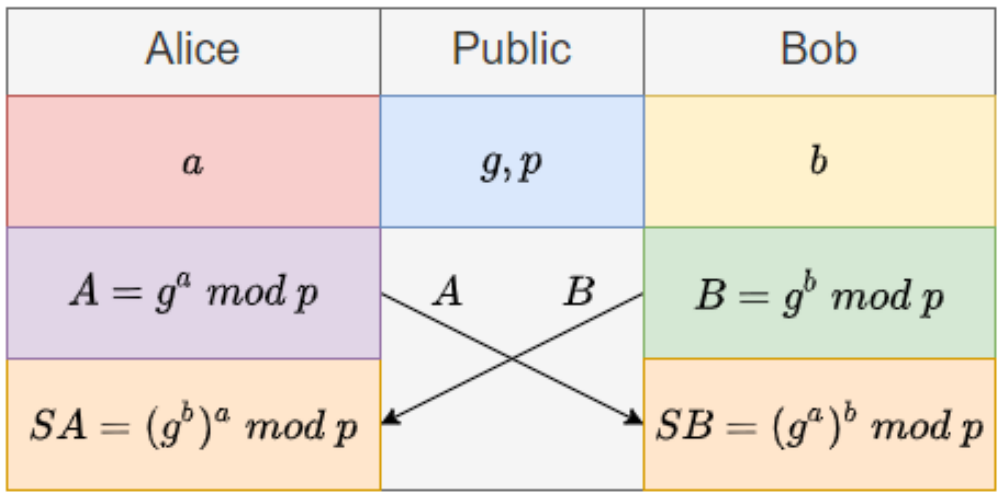
\includegraphics[width=\linewidth]{diffie_hellman_diagram.png}

\begin{remark}
    The secret may not be suitable for to use as a symmetric key:
    \begin{itemize}
        \item Some bits may always be zero or one
        \item The secret may be too long or too short
    \end{itemize}
    
    The secret is put through a key derivation function (KDF) to get the key.
\end{remark}

\subsubsection{Problems with Diffie-Hellman}

\begin{concept}{DH Limitations}
    \begin{itemize}
        \item What if Bob and Alice are not speaking to each other?
        \item Eve can make a Man-in-the-Middle Attack.
        \item Bob and Alice need to be Online.
    \end{itemize}
\end{concept}


\begin{concept}{Integrated Encryption Scheme (IES)}
    Solves Offline Problem (of DH)
\end{concept}

\raggedcolumns
\columnbreak

\section{Data Integrity and Authentication}



\subsection{Kryptographische Hash Funktionen}

\begin{definition}{Kryptographische Hash Funktion} ist eine mathematische Funktion mit folgenden Eigenschaften:
    \begin{itemize}
        \item aus einem beliebig langen Input wird Output mit konstanter Länge generiert
        \item es gibt keine Möglichkeit aus dem Output den Input wieder herzuleiten
        \item unterschiedliche Inputs ergeben mit sehr hoher Wahrscheinlichkeit völlig unterschiedliche Outputs, auch wenn sich die Inputs nur wenig unterscheiden
        \item es ist nicht möglich innert nützlicher Zeit zwei unterschiedliche Inputs zu generieren, welche denselben Output haben
    \end{itemize}

    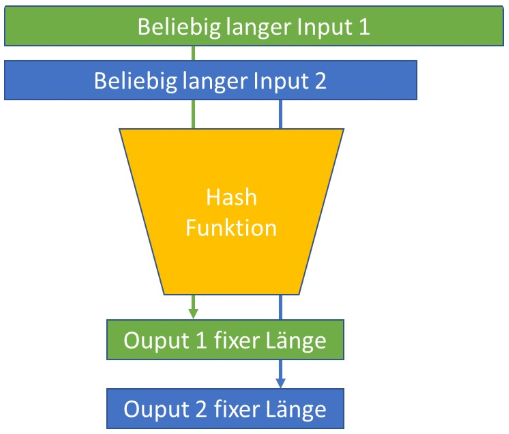
\includegraphics[width=0.6\linewidth]{krypto_hashfunktionen.png}
    
\end{definition}

\begin{concept}{Important Properties}
    \begin{itemize}
        \item \textbf{Efficient computation}
        \item \textbf{Pseudo-random}
        \item \textbf{Preimage resistance} Given a hash, it is practically impossible to find a massage that produces the hash
        \item \textbf{Collision resistance} It is practically impossible to find any two messages that map to the same hash
    \end{itemize}
    
    A hash function should behave like a random oracle. Different inputs $\rightarrow$ totally unrelated outputs.
\end{concept}

\begin{formula}{Work Factor}
    Da bei Hash Funktionen der Output weniger lang ist als der Input gibt es keinen Algorithmus, welcher für alle Inputs und Outputs die Eigenschaften 3 und 4 erreicht. Das heisst, es wird immer verschiedene Inputs geben, welche denselben Output generieren. Mit dem Work Faktor kann angegeben werden, wie gross der Aufwand ist, um diese Hash Collisions zu berechnen.

Der Work Faktor in bits einer kryptographischen Funktion entspricht der Hälfte der bits des generierten Outputs.

Auch hier gilt: Für eine sichere Hash Funktion sollte der Work Faktor mindestens 128 bit betragen.    
\end{formula}

\raggedcolumns
\columnbreak


\subsection{Password Security}





\begin{concept}{Password Authentication} Popular, easy to implement, changeable
\end{concept}

\mult{2}

\begin{definition}{Password security problems}
    \begin{itemize}
        \item \textbf{Sniffing} Passwords are transmitted in plaintext $\rightarrow$ Prevent with Protected links (TLS)
        \item \textbf{Phishing} Show fake login screen to capture password $\rightarrow$ Prevent with Certificates
        \item \textbf{Online Attacks} Password guessing $\rightarrow$ Prevent with Slowdown / blocking
        \item \textbf{Offline Attacks} Compromises system and gets pw from db $\rightarrow$ Do not save passwords in plaintext
        \item \textbf{Password Re-use} Remove password-strength
    \end{itemize}
\end{definition}

\begin{KR}{Cracking Hashed passwords}

    \textbf{Step 1: Dictionary Attack}
    Try passwords and compute the hash and check if fit matches any hash in the password file
    
    \textbf{Step 2: Strategic Testing}
    Test strategically with Dictionary attack, Minor variations...
    
    \textbf{Step 3: Precompiled Attack}
    Compute a huge list of passwords and hashes (beforehand)
\end{KR}

\begin{concept}{Message Tampering Detection}
    \begin{itemize}
        \item Use a hash function together with a secret key (Message Authentication Code)
        \item Use a hash function together with digital signatures
    \end{itemize}
\end{concept}

\begin{concept}{Salting} Protect password hashes\\
    Add a random value called salt before hashing to prevent precompiled attacks.

    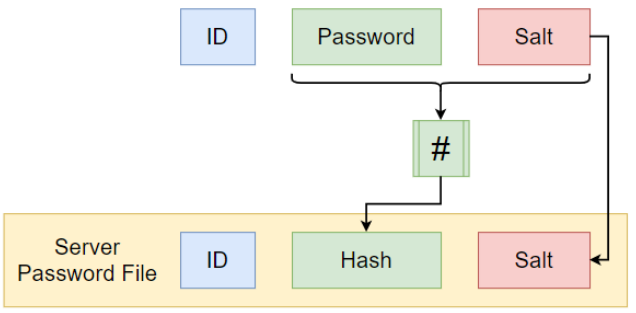
\includegraphics[width=0.8\linewidth]{protect_pw_hashes.png}
\end{concept}

\begin{formula}{Hash Collision Probability}
    $n = HashLength$ (in bits)
    \begin{itemize}
        \item Two random Hashes: $2^{n/2}$
        \item Collision with given Hash: $2^{n-1}$
    \end{itemize}
\end{formula}

\multend

\subsubsection{Message Authentication Codes (MAC) = Message Integrity Check (MIC)}

\begin{definition}{MAC Purpose}
    The idea is to use a key in addition to the hash function to prevent an attacker from changing the message and calculating a new hash...
\end{definition}



\begin{KR}{MAC Workflow (Using Secret Key Cryptography)}

    \begin{minipage}{0.5\linewidth}
    \textbf{Step 1} Alice Send document

    \textbf{Step 2} Bob Apply "Keyed Hash Function" = $MAC_1$

    \textbf{Step 3} Alice Apply "Keyed Hash Function" = $MAC_2$

    \textbf{Step 4} Alice Send $MAC_2$

    \textbf{Step 5} Bob Compare $MAC_1$ and $MAC_2$
    \end{minipage}
    \begin{minipage}{0.5\linewidth}
        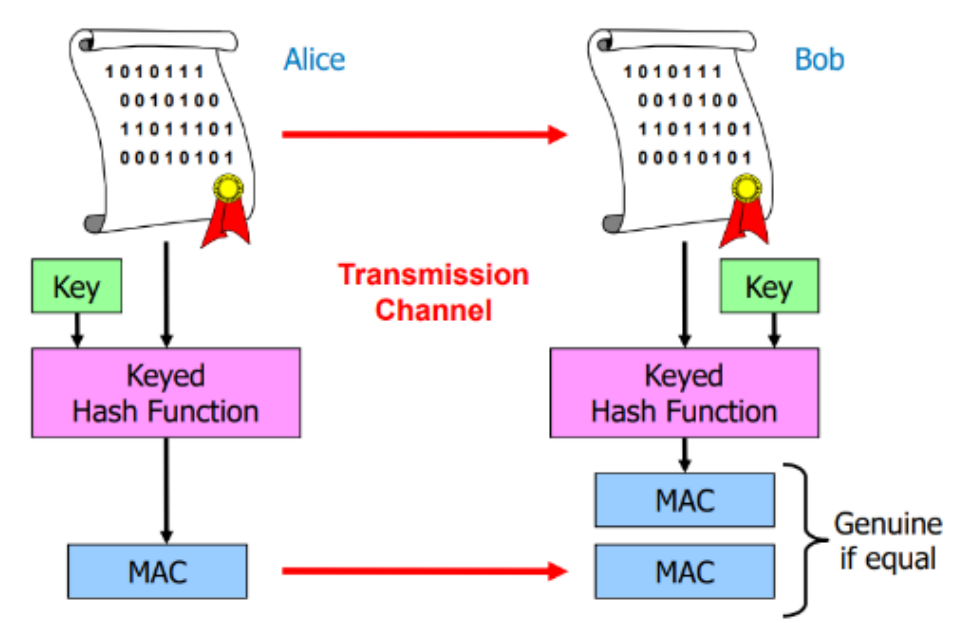
\includegraphics[width=0.8\linewidth]{MAC.png}
    \end{minipage}
\end{KR}

\begin{concept}{HMAC}

    \begin{minipage}{0.5\linewidth}
    HMAC is a concrete implementation of the MAC concept.
    \begin{itemize}
        \item Generate Inner $K_I$ and Outer Key $K_O$
        \item Hash $H(K_I, M) = H_1$
        \item Hash $H(K_O, M) = H_2 = MAC$
        \item Keyed Hash Function: $H(K_O, H(K_I, M))$
    \end{itemize}
    \end{minipage}
    \begin{minipage}{0.5\linewidth}
    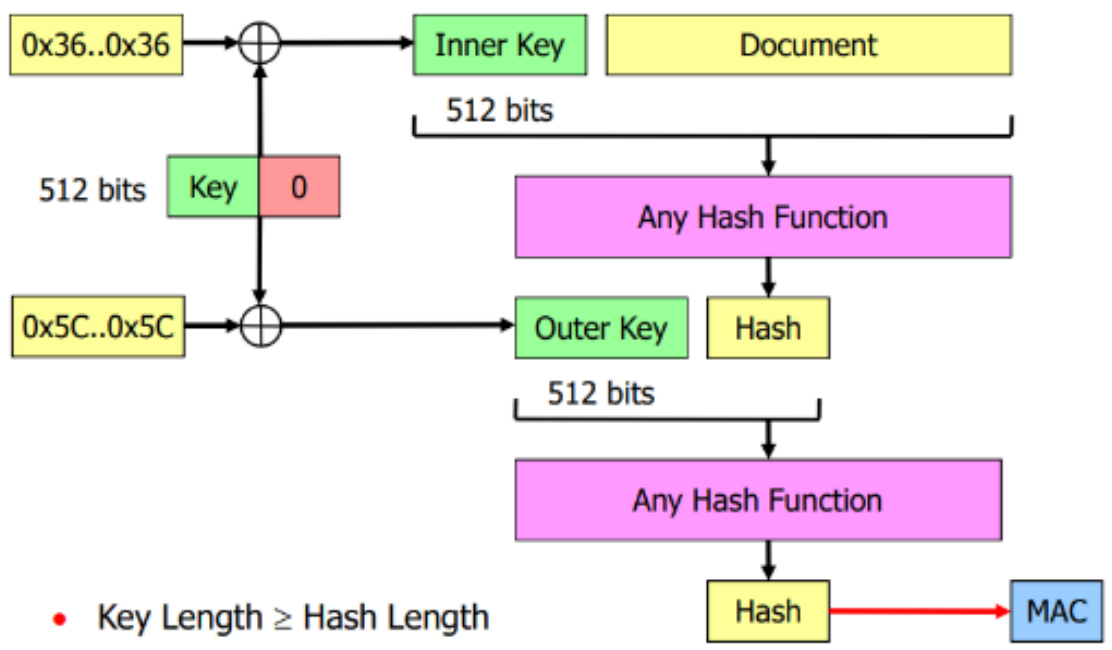
\includegraphics[width=\linewidth]{HMAC.png}
    \end{minipage}
\end{concept}



\subsubsection{Digital Signature}

\begin{KR}{Digital Signature Workflow (Using Public Key Cryptography)}

    \begin{minipage}{0.5\linewidth}
    \textbf{Step 1} Signer Send document $M$

    \textbf{Step 2} Verifier Hash document $M \rightarrow H(M) = X$

    \textbf{Step 3} Signer Hash document $M \rightarrow H(M)$

    \textbf{Step 4} Signer Encrypt document $H(M) \rightarrow E(H(M))$

    \textbf{Step 5} Signer Send document $E(H(M))$

    \textbf{Step 6} Verifier Decrypt document $D(H(M)) \rightarrow H(M) = Y$

    \textbf{Step 7} Verifier Compare hashes $X == Y$
    \end{minipage}
    \begin{minipage}{0.5\linewidth}
        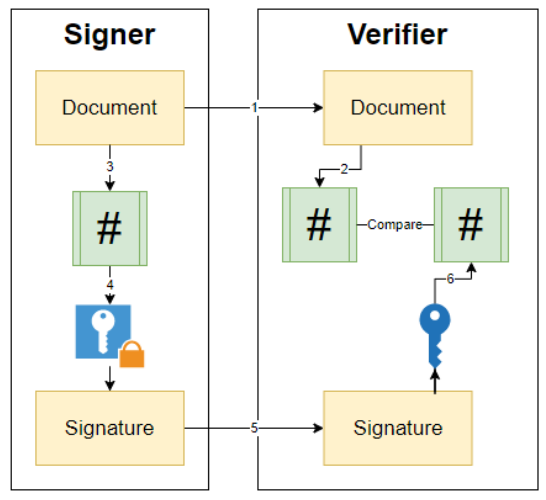
\includegraphics[width=0.8\linewidth]{digital_signature.png}
    \end{minipage}
\end{KR}



\subsubsection{Galois Counter mode (GCM)}

\begin{concept}{GCM}
    Only encrypting a message doesn't provide Integrity Protection $\rightarrow$ GCM
    \begin{itemize}
        \item Combine Integrity and Encryption
        \item Approach «Encrypt then MAC»
    \end{itemize}
\end{concept}

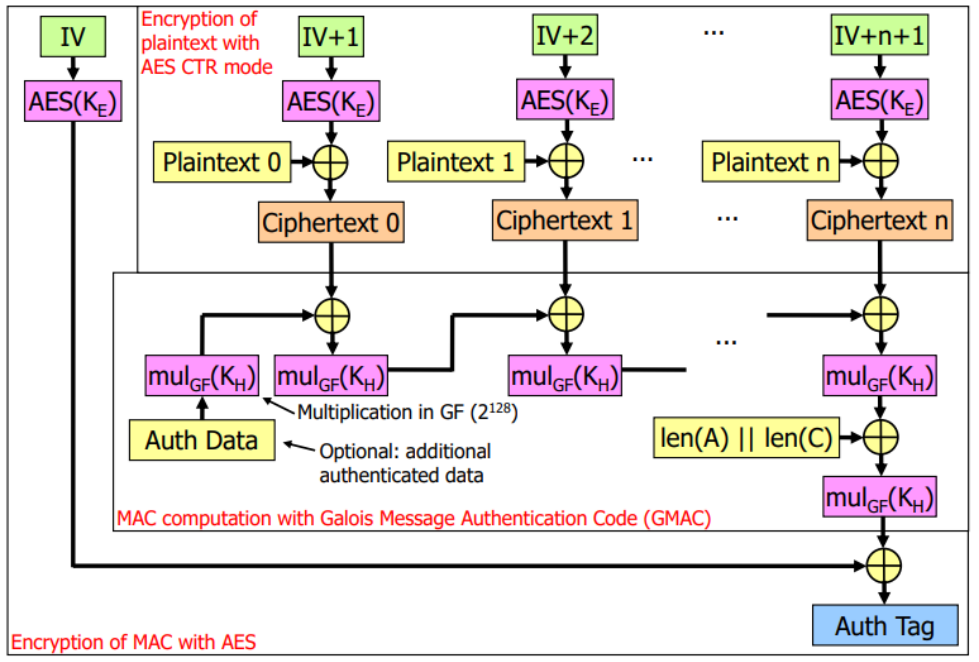
\includegraphics[width=0.8\linewidth]{GCM.png}

\subsubsection{Comparison: MAC vs Digital Signatures}

\mult{2}

\begin{concept}{MAC}
    \begin{itemize}
        \item Fast and efficient
        \item Receiver must know the secret key
    \end{itemize}
\end{concept}

\begin{concept}{Digital Signatures}
    \begin{itemize}
        \item Public key is openly available
        \item En- / Decryption are time intensive
    \end{itemize}
\end{concept}

\multend